% Provenance (never printed): old terminale S material on absolute dating (the
% decay law recalled, the closed system, the rubidium-strontium isochron) and on
% the history of the age of the Earth (cooling, salt, sediments, then radioactivity,
% meteorites and 4.55 billion years). Owner (Sync 0/1): closed system, isochron,
% age of the Earth (as a defined notion). The decay law, the half-life and the
% dating equation are the physics books' (recalled); relative dating, absolute
% age, superposition, cross-cutting relationships and the eras are Book 1 g7's
% (recalled); the oldest zircons and the Acasta gneiss are g12.01's (quoted).
% Varden Hills granite 310 Ma and schist 480 Ma from figdata/shared/region.py;
% their isotope ratios are exercise data (figdata/grade-12/isochrons.py).
\chapter{La datación radiométrica y la edad de la Tierra}\label{ch:g12:age-of-the-earth}

En 1862, el físico William Thomson, más tarde lord Kelvin, calculó la \omterm{def:g12:age-of-the-earth:age}{edad de
la Tierra} a partir de su forma de enfriarse. Supuso que se había formado
fundida y que desde entonces había ido perdiendo su calor, y se preguntó
cuánto tiempo tardaría el gradiente de temperatura cerca de la superficie en
bajar hasta su valor actual. Su respuesta fue 96 millones de años, entre 20 y
400 millones; en 1897 había reducido el intervalo a entre 20 y 40 millones.
Los geólogos lo consideraron demasiado corto para la historia que leían en las
rocas. La respuesta llegó de la radiactividad, que Kelvin no conocía.
% ledger: holmes13:estimates, england:kelvin (Book 3 row)

\begin{omfigure}
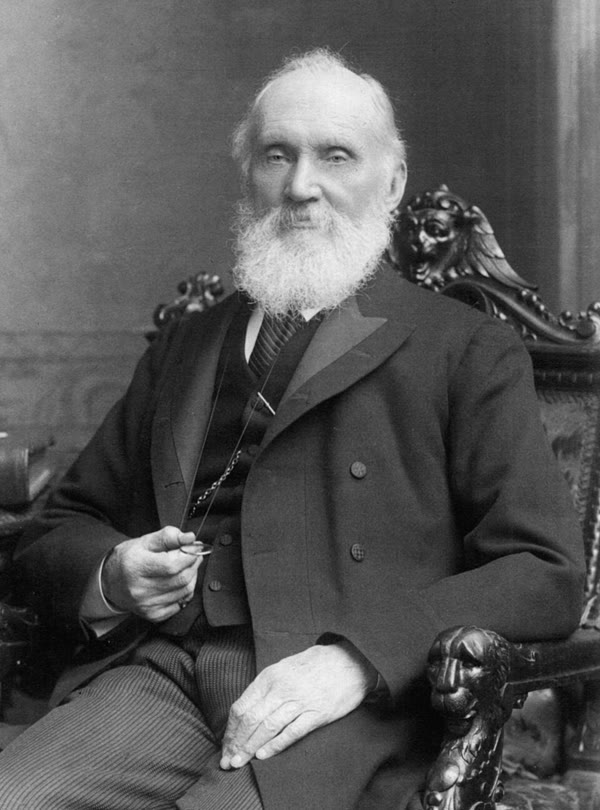
\includegraphics[height=5.2cm]{images/book2/g12-kelvin-1906.jpg}

{\small William Thomson, lord Kelvin, en 1906. Fotografía de Russell and Sons,
Londres (Smithsonian Institution Libraries, sin restricciones de derechos
conocidas).}
\end{omfigure}
% ledger: photo:g12-kelvin

\begin{recall}
La datación relativa ordena las rocas y los sucesos; una edad absoluta es un
número de años (Libro 1, año 7). Un isótopo radiactivo, el padre, se
desintegra al azar en un isótopo hijo: el número $N$ de átomos padre que
quedan disminuye según
$N = N_0\,e^{-\lambda t}$, donde $\lambda$ es la constante de desintegración,
y se reduce a la mitad en cada periodo de semidesintegración $T = \ln 2/\lambda$ (los libros de física). Los minerales más antiguos que se
conocen, unos circones de Australia Occidental, tienen 4400 millones de años
(el \cref{ch:g12:continental-crust}). La Tierra pierde además un calor que la
radiactividad sigue produciendo, y su manto tiene convección (el
\cref{ch:g12:internal-heat}).
\end{recall}
% ledger: wilde01:zircon

\section{Una historia de estimaciones}

Antes de la radiactividad, cada estimación de la \omterm{def:g12:age-of-the-earth:age}{edad de la Tierra} se basaba
en un proceso cuyo ritmo se suponía conocido.

\begin{center}
\small
\begin{tabular}{|p{0.19\linewidth}|p{0.42\linewidth}|p{0.25\linewidth}|}
\hline
quién, cuándo & método y lo que supone & estimación \\
\hline
Phillips, 1860 & espesor de las capas sedimentarias dividido por un ritmo de sedimentación; supone un ritmo constante & de 38 a 96 millones de años \\
Kelvin, 1862 & enfriamiento por conducción, sin más, de una Tierra fundida, sin ninguna fuente de calor en su interior & de 20 a 400 millones de años \\
G.\,H.~Darwin & tiempo transcurrido desde que la Luna se separó de la Tierra, a partir del frenado de sus movimientos por las mareas & al menos 56 millones de años \\
Joly, 1899 & sal llevada al mar por los ríos, dividida por el aporte anual; supone un aporte constante y que no se retira sal & de 80 a 100 millones de años \\
\hline
\end{tabular}
\end{center}
% ledger: holmes13:estimates

\begin{history}[El calor que le faltaba a Kelvin]
En 1903, Pierre Curie y Albert Laborde mostraron que el radio desprende
calor, y varios científicos sostuvieron pronto que ese calor echaba por
tierra la conclusión de Kelvin. Un año después, Ernest Rutherford, en una
conferencia con Kelvin entre el público, le recordó que había limitado la
\omterm{def:g12:age-of-the-earth:age}{edad de la Tierra} ``siempre que no se descubriera ninguna nueva fuente de
calor''. La radiactividad parecía ser esa fuente. Sin embargo, no fue el error
principal de Kelvin: lo que más alarga el enfriamiento de la Tierra es la
\omterm{def:g12:internal-heat:convection}{convección del manto}, que mantiene caliente el manto superior y alto el
gradiente de la corteza durante mucho más tiempo del que lo haría la
conducción sola.
\end{history}
% ledger: england:kelvin (Book 3 row)

La radiactividad aportó además un reloj. En 1907, Bertram Boltwood mostró que
los minerales de uranio de la misma edad contienen la misma cantidad de plomo
por cada gramo de uranio: el plomo lo produce el uranio. En 1913, Arthur
Holmes pudo escribir que las rocas más antiguas datadas tenían \num{1600}
millones de años, y en 1927 situó la \omterm{def:g12:age-of-the-earth:age}{edad de la Tierra} entre 1600 y 3000
millones de años. En 1956, Clair Patterson midió 4550 millones de años. El
valor actual es de 4540 millones de años, con un margen de un uno por ciento.
% ledger: holmes13:estimates, holmes27:age, patterson56:table, usgs:age-earth (Book 1 row)

\begin{omfigure}
\begin{tikzpicture}
\begin{axis}[omrecord, width=0.78\linewidth, height=6.2cm, ymode=log, xmin=1840, xmax=2040,
  ymin=1e7, ymax=2e10, xlabel={año de la estimación}, ylabel={edad estimada de la Tierra (años)},
  xtick={1850,1875,...,2025}, x tick label style={/pgf/number format/.cd, set thousands separator={}},
  ytick={1e7,1e8,1e9,1e10}, ymajorgrids=true, xmajorgrids=false]
% computed in figdata/grade-12/isochrons.py; ledger: holmes13:estimates, holmes27:age, patterson56:table, usgs:age-earth (Book 1 row)
\addplot[omDef, only marks, mark=*, mark size=1.8pt, error bars/.cd, y dir=both, y explicit]
  table[x=year, y=mid, y error minus expr=\thisrow{mid}-\thisrow{lo}, y error plus expr=\thisrow{hi}-\thisrow{mid}]
  {figdata/out/grade-12-isochrons-history.dat};
\addplot[omThm, densely dashed, domain=1840:2040, samples=2] {4.54e9};
\coordinate (k62) at (axis cs:1862,2.4e8);
\coordinate (k97) at (axis cs:1897,2.8e7);
\coordinate (jol) at (axis cs:1899,1e8);
\coordinate (h11) at (axis cs:1919,1.3e9);
\coordinate (pat) at (axis cs:1956,4.55e9);
\coordinate (now) at (axis cs:1845,4.54e9);
\end{axis}
\node[font=\scriptsize, anchor=west] at ([xshift=4pt]k62) {Kelvin 1862};
\node[font=\scriptsize, anchor=east] at ([xshift=-4pt]k97) {Kelvin 1897};
\node[font=\scriptsize, anchor=west] at ([xshift=4pt]jol) {Joly};
\node[font=\scriptsize, anchor=north] at (h11) {Holmes};
\node[font=\scriptsize, anchor=north west] at ([xshift=2pt, yshift=-3pt]pat) {Patterson};
\node[font=\scriptsize, text=omThm, anchor=south west] at (now) {hoy, 4540 millones de años};
\end{tikzpicture}

{\small Estimaciones de la \omterm{def:g12:age-of-the-earth:age}{edad de la Tierra} frente al año en que se hicieron,
en escala logarítmica; las barras abarcan el intervalo que dio cada autor. El
punto de Holmes de 1913 es la edad de las rocas más antiguas datadas
entonces, un mínimo. Fuentes: Holmes (1913, 1927); Patterson (1956); Servicio
Geológico de los Estados Unidos.}
\end{omfigure}

\section{Un reloj radiactivo}

Un reloj radiactivo solo funciona si no se le ha añadido ni quitado nada
desde que se puso en marcha.

\begin{definition}[Sistema cerrado]\label{def:g12:age-of-the-earth:closed-system}
Una roca o un mineral es un \emph{sistema cerrado}\index{sistema cerrado} para
un isótopo padre y su hijo si, desde el momento en que su reloj se puso en
marcha, ningún átomo del padre ni del hijo ha entrado en él ni ha salido de
él, salvo por la desintegración del padre en el hijo.
\end{definition}
% ledger: tulane:radiometric

En un mineral, el reloj se pone en marcha cuando cristaliza a partir de un
magma o, más exactamente, cuando se ha enfriado lo suficiente para que los
átomos dejen de entrar y salir de él. Un calentamiento, un fluido caliente o
la meteorización pueden volver a abrir el sistema, y la edad que se mide
entonces es falsa, o data ese suceso posterior.
% ledger: tulane:radiometric

Contar los átomos hijos de un \omterm{def:g12:age-of-the-earth:closed-system}{sistema cerrado} da la edad, siempre que se sepa
cuántos había al principio. Normalmente no se sabe. El rubidio 87 se
desintegra en estroncio 87, pero cada mineral incorporó también algo de
estroncio 87 al formarse. El método de la \omterm{def:g12:age-of-the-earth:isochron}{isócrona} resuelve esto midiendo
varios minerales de una misma roca.

\section{La isócrona}

El estroncio tiene un isótopo, el estroncio 86, que es estable y no procede
de ninguna desintegración: en un \omterm{def:g12:age-of-the-earth:closed-system}{sistema cerrado} su número no cambia, y sirve
de patrón. Las razones isotópicas $^{87}\mathrm{Sr}/^{86}\mathrm{Sr}$ y
$^{87}\mathrm{Rb}/^{86}\mathrm{Sr}$ son lo que mide un espectrómetro de masas.

\begin{theorem}[La ecuación de la isócrona]\label{thm:g12:age-of-the-earth:isochron}
En un mineral que ha sido un \omterm{def:g12:age-of-the-earth:closed-system}{sistema cerrado} durante un tiempo $t$,
\[
  \left(\frac{^{87}\mathrm{Sr}}{^{86}\mathrm{Sr}}\right)_{\text{hoy}}
  = \left(\frac{^{87}\mathrm{Sr}}{^{86}\mathrm{Sr}}\right)_{0}
  + \left(\frac{^{87}\mathrm{Rb}}{^{86}\mathrm{Sr}}\right)_{\text{hoy}}
  \left(e^{\lambda t} - 1\right),
\]
donde el índice 0 indica el valor cuando el reloj se puso en marcha y
$\lambda$ es la constante de desintegración del rubidio 87.
\end{theorem}

\begin{proof}
Sea $P$ el número de átomos de rubidio 87 hoy y $P_0$ cuando el reloj se puso
en marcha. Según la ley de desintegración, $P = P_0\,e^{-\lambda t}$, así que $P_0 = P\,e^{\lambda t}$,
y el número de átomos que se han desintegrado es $P_0 - P = P\,(e^{\lambda t}-1)$.
En un \omterm{def:g12:age-of-the-earth:closed-system}{sistema cerrado}, cada uno de ellos se ha convertido en un átomo de
estroncio 87, que se suma a los $D_0$ átomos presentes al principio: $D = D_0 + P\,(e^{\lambda
t}-1)$. Dividiendo por el número de átomos de estroncio 86, que no ha
cambiado, se obtiene la ecuación.
\end{proof}
% ledger: tulane:radiometric

Los minerales de un granito cristalizaron a partir de un mismo magma, así que
todos empezaron con la misma razón $(^{87}\mathrm{Sr}/^{86}\mathrm{Sr})_0$.
Pero incorporaron cantidades muy distintas de rubidio. Como todos comparten el
mismo $t$ y la misma razón inicial, la ecuación dice que sus puntos están
sobre una misma recta.

\begin{definition}[Isócrona]\label{def:g12:age-of-the-earth:isochron}
Una \emph{isócrona}\index{isocrona@isócrona} es la recta sobre la que se
encuentran los puntos de minerales o rocas que se formaron al mismo tiempo a
partir de la misma fuente y han seguido siendo \omterm{def:g12:age-of-the-earth:closed-system}{sistemas cerrados} desde
entonces, cuando se representa la razón del isótopo hijo al isótopo estable
frente a la razón del isótopo padre al isótopo estable. Su pendiente da su
edad, y el punto donde corta el eje vertical da su razón inicial.
\end{definition}
% ledger: tulane:radiometric

\begin{proposition}[La edad a partir de la pendiente]\label{prop:g12:age-of-the-earth:slope}
Si una \omterm{def:g12:age-of-the-earth:isochron}{isócrona} tiene una pendiente $m$, la edad es
\[
  t = \frac{\ln(1+m)}{\lambda}.
\]
\end{proposition}

\begin{proof}
Comparando con la ecuación de la \omterm{def:g12:age-of-the-earth:isochron}{isócrona}, $m = e^{\lambda t} - 1$, así que
$e^{\lambda t} = 1 + m$, $\lambda t = \ln(1+m)$, y $t = \ln(1+m)/\lambda$.
\end{proof}

Para el rubidio 87, $\lambda = \num{1.3972e-11}$ por año, un periodo de
semidesintegración de
$\ln 2/\lambda \approx 49.6$ mil millones de años: más de diez veces la \omterm{def:g12:age-of-the-earth:age}{edad
de la Tierra}.
% ledger: villa22:rb87

\begin{method}[Datar una roca con una isócrona]\label{met:g12:age-of-the-earth:isochron}
\begin{enumerate}
  \item Separa varios minerales de la roca (o toma varias muestras de ella)
        con cantidades distintas de rubidio.
  \item Mide en cada uno las razones $^{87}\mathrm{Rb}/^{86}\mathrm{Sr}$ ($x$)
        y $^{87}\mathrm{Sr}/^{86}\mathrm{Sr}$ ($y$).
  \item Representa $y$ frente a $x$ y comprueba que los puntos están sobre una
        recta: si uno no lo está, esa muestra no fue un \omterm{def:g12:age-of-the-earth:closed-system}{sistema cerrado}.
  \item Toma la pendiente $m$ de la recta y calcula $t = \ln(1+m)/\lambda$.
  \item Lee la razón inicial donde la recta corta el eje vertical.
\end{enumerate}
\end{method}

\begin{example}[El granito de Varden]\label{ex:g12:age-of-the-earth:varden}
El granito de las Varden Hills, la región inventada de la serie, da estas
razones (datos de ejercicio):
\begin{center}
\small
\begin{tabular}{|l|c|c|}
\hline
muestra & $^{87}\mathrm{Rb}/^{86}\mathrm{Sr}$ & $^{87}\mathrm{Sr}/^{86}\mathrm{Sr}$ \\
\hline
plagioclasa & 0.35 & 0.70952 \\
hornblenda  & 1.20 & 0.71321 \\
roca total  & 3.10 & 0.72146 \\
feldespato K  & 6.40 & 0.73578 \\
biotita     & 24.0 & 0.81218 \\
\hline
\end{tabular}
\end{center}
A través de la plagioclasa y la biotita, la pendiente es
$m = (0.81218 - 0.70952)/(24.0 - 0.35) \approx 0.004341$. Entonces
$t = \ln(1.004341)/\num{1.3972e-11} \approx \num{3.10e8}$ años:
el granito tiene 310 millones de años. La recta corta el eje vertical en
$0.70952 - 0.35 \times 0.004341 \approx 0.7080$, la razón inicial.
\end{example}
% values: granite_age_Ma 310.0, granite_intercept 0.70800 (isochrons.py)

\begin{omfigure}
\begin{tikzpicture}
\begin{axis}[omrecord, width=0.7\linewidth, height=6cm, xmin=0, xmax=26, ymin=0.695, ymax=0.82, ytick={0.70,0.72,...,0.82},
  xlabel={$^{87}\mathrm{Rb}/^{86}\mathrm{Sr}$}, ylabel={$^{87}\mathrm{Sr}/^{86}\mathrm{Sr}$},
  y tick label style={/pgf/number format/.cd, fixed, fixed zerofill, precision=2}]
% computed in figdata/grade-12/isochrons.py (exercise data, Varden granite 310 Ma); ledger: villa22:rb87
\addplot[omDef, line width=0.9pt] table[x=x, y=y] {figdata/out/grade-12-isochrons-graniteln.dat};
\addplot[omThm, only marks, mark=*, mark size=2pt] table[x=rbsr, y=srsr] {figdata/out/grade-12-isochrons-granite.dat};
\addplot[black!60, densely dotted, domain=0:26, samples=2] {0.7080};
\coordinate (pl) at (axis cs:0.35,0.70952);
\coordinate (hb) at (axis cs:1.2,0.71321);
\coordinate (wr) at (axis cs:3.1,0.72146);
\coordinate (kf) at (axis cs:6.4,0.73578);
\coordinate (bt) at (axis cs:24,0.81218);
\coordinate (sl) at (axis cs:12,0.762);
\coordinate (in) at (axis cs:9,0.7082);
\coordinate (plhb) at (axis cs:0.6,0.737);
\coordinate (plhbpt) at (axis cs:0.9,0.7125);
\end{axis}
\node[font=\scriptsize, anchor=north west] at ([xshift=1pt]wr) {roca total};
\node[font=\scriptsize, anchor=north west] at ([xshift=1pt]kf) {feldespato K};
\node[font=\scriptsize, anchor=east] at ([xshift=-3pt]bt) {biotita};
\node[font=\scriptsize, anchor=south west, align=left, inner sep=1pt] (plhblab) at (plhb) {plagioclasa,\\hornblenda};
\draw[black!60, line width=0.4pt] (plhblab.south) -- (plhbpt);
\node[font=\scriptsize, text=omDef, anchor=south east] at (sl) {\shortstack[r]{pendiente $0.004341$:\\310 millones de años}};
\node[font=\scriptsize, text=black!70, anchor=south west] at (in) {razón inicial 0.7080 (tiempo 0)};
\end{tikzpicture}

{\small La \omterm{def:g12:age-of-the-earth:isochron}{isócrona} rubidio--estroncio del granito de Varden (datos de
ejercicio). Cuando se formó el granito, todos sus minerales estaban sobre la
recta horizontal punteada; desde entonces, cada uno ha subido en proporción a
su rubidio, y ahora están sobre la recta continua.}
\end{omfigure}

\begin{inthelab}[Pesar átomos]
Las razones se miden con un espectrómetro de masas. Se disuelven en ácido
unos miligramos de un mineral, y el estroncio se separa del rubidio por vía
química, ya que si no se contarían juntos los dos isótopos de masa 87. El
estroncio, depositado sobre un filamento metálico y calentado en el vacío,
emite iones; un campo eléctrico los acelera y un imán curva sus trayectorias,
más las de los iones ligeros que las de los pesados, de modo que cada isótopo
llega a su propio colector. Sus corrientes dan las razones.
\end{inthelab}

\begin{omfigure}
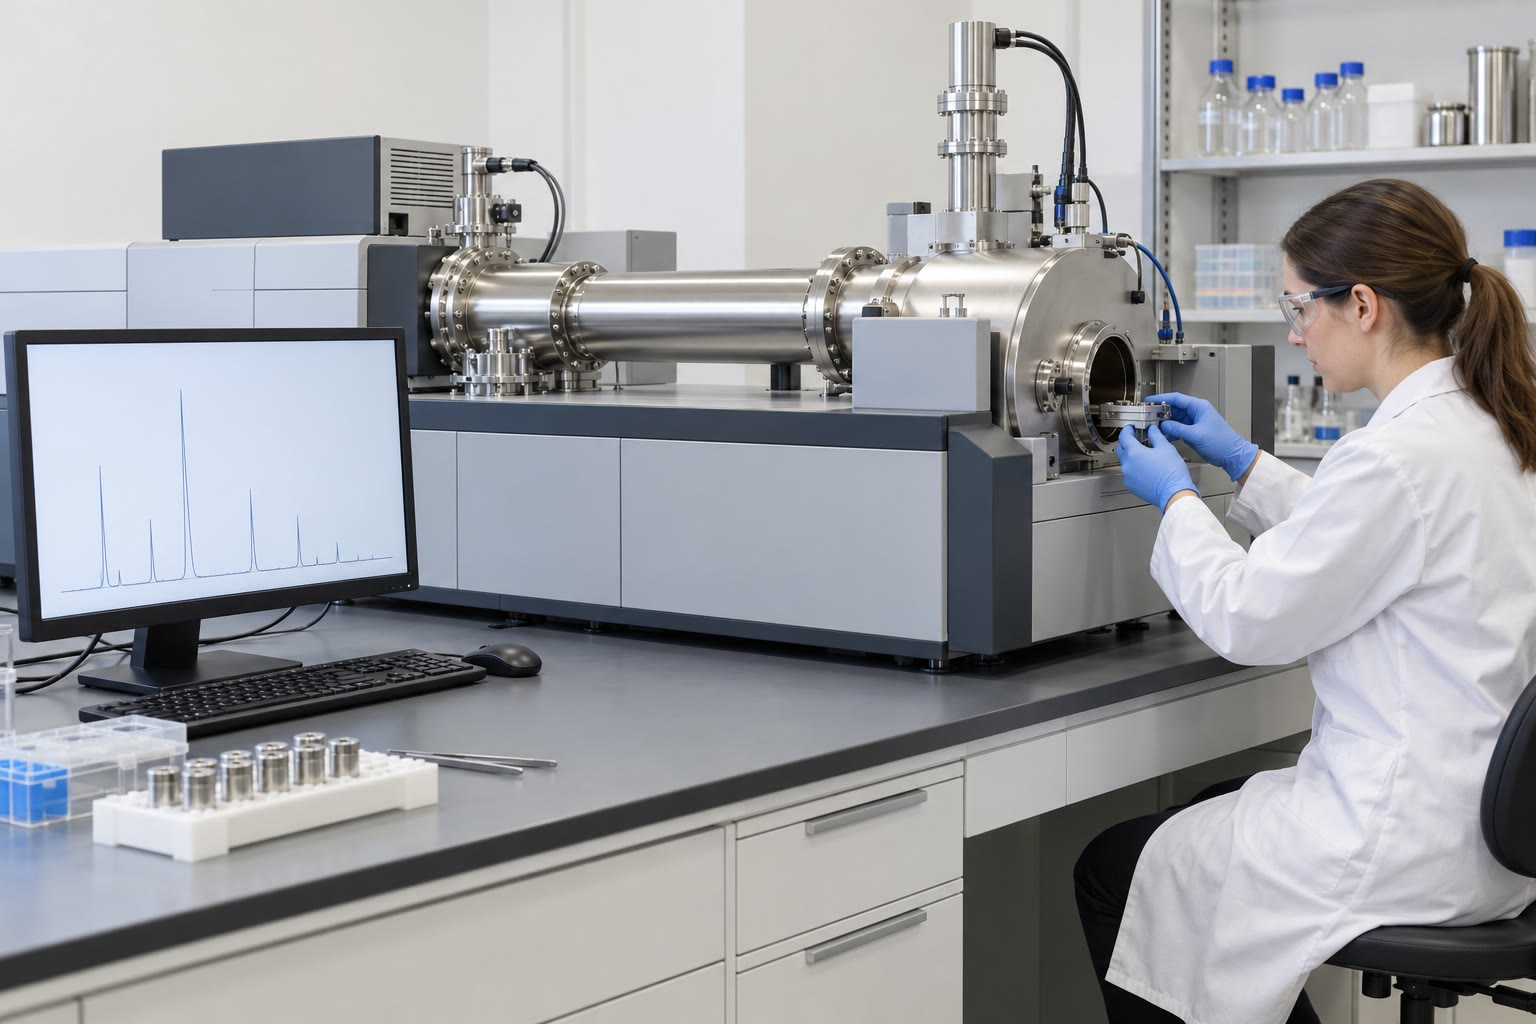
\includegraphics[width=0.66\linewidth]{images/book2/ai/g12-mass-spectrometer-lab.jpg}

{\small Un espectrómetro de masas en un laboratorio: se está cargando una
muestra en el extremo de la fuente. Ilustración generada por IA.}
\end{omfigure}

La razón inicial es también una pista sobre el origen del magma. El rubidio
prefiere el fundido cuando el manto se funde, así que con las eras se ha
concentrado en la \omterm{def:g12:continental-crust:continental-crust}{corteza continental}, que por eso ha producido más
estroncio 87: las rocas de la corteza tienen una razón
$^{87}\mathrm{Sr}/^{86}\mathrm{Sr}$ más alta que las del manto. Un magma
procedente de corteza fundida hereda esa razón alta.
% ledger: tulane:radiometric

\section{La edad de la Tierra}

Ninguna roca de la Tierra se remonta al origen del planeta: la roca más
antigua que se conoce, el gneis de Acasta, tiene 4030 millones de años, y los
circones más antiguos, 4400 millones. La superficie se ha fundido, erosionado
y reciclado desde entonces. La datación de la propia Tierra procede de los
meteoritos, fragmentos de los pequeños cuerpos que se formaron con los
planetas, algunos de los cuales han seguido siendo \omterm{def:g12:age-of-the-earth:closed-system}{sistemas cerrados} desde
entonces.
% ledger: bowring99:acasta, wilde01:zircon, usgs:age-earth (Book 1 row)

\begin{definition}[Edad de la Tierra]\label{def:g12:age-of-the-earth:age}
La \emph{edad de la Tierra}\index{edad de la Tierra} es el tiempo transcurrido
desde que la Tierra se formó por acreción de cuerpos más pequeños, en el
nacimiento del sistema solar. Medida en meteoritos por datación radiométrica,
es de \num{4.54}~mil millones de años, con un margen de un uno por ciento.
\end{definition}
% ledger: usgs:age-earth (Book 1 row)

En 1956, Clair Patterson midió los isótopos del plomo en tres meteoritos
rocosos y dos meteoritos metálicos. Dos isótopos del plomo proceden de la
desintegración del uranio, el plomo 206 del uranio 238 y el plomo 207 del
uranio 235, mientras que el plomo 204 no procede de ninguna desintegración.
Como con el estroncio, los puntos de los meteoritos que se formaron al mismo
tiempo están sobre una recta cuando se representa
$^{207}\mathrm{Pb}/^{204}\mathrm{Pb}$ frente a
$^{206}\mathrm{Pb}/^{204}\mathrm{Pb}$. El meteorito metálico de Canyon Diablo,
en Arizona, casi no contiene uranio: su plomo no ha cambiado desde que se
formó, y marca el extremo inferior de la recta, el plomo con el que empezó el
sistema solar.
% ledger: patterson56:table, patterson56:constants, usgs:age-earth (Book 1 row: Canyon Diablo troilite)

\begin{omfigure}
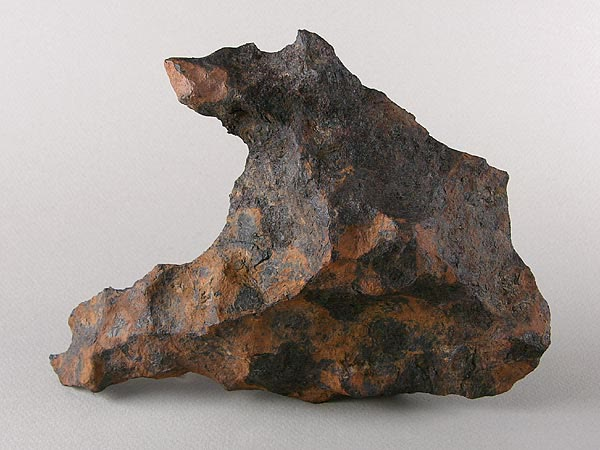
\includegraphics[height=4.2cm]{images/book2/g12-canyon-diablo-meteorite.jpg}

{\small Un fragmento del meteorito metálico de Canyon Diablo, \qty{2641}{g}.
Fotografía de Geoffrey Notkin, CC~BY-SA~2.5 (Wikimedia Commons).}
\end{omfigure}
% ledger: photo:g12-canyon-diablo

Para el plomo, la pendiente $m$ depende de la edad a través de los dos
isótopos del uranio; la relación se admite aquí. Con las constantes que usó
Patterson,
\[
  m = \frac{1}{137.8}\,\frac{e^{\lambda_{235}t}-1}{e^{\lambda_{238}t}-1},
  \qquad \lambda_{235} = \num{9.72e-10},\ \lambda_{238} = \num{1.537e-10}
  \text{ por año},
\]
lo que da:
\begin{center}
\small
\begin{tabular}{|l|c|c|c|c|c|c|}
\hline
edad (miles de millones de años) & 4.40 & 4.45 & 4.50 & 4.55 & 4.60 & 4.65 \\
pendiente $m$ & 0.533 & 0.551 & 0.570 & 0.590 & 0.610 & 0.632 \\
\hline
\end{tabular}
\end{center}
% ledger: patterson56:constants
% values: pb_slope at 4.40-4.65 Ga (isochrons.py pb_slope)

\begin{omfigure}
\begin{tikzpicture}
\begin{axis}[omrecord, width=0.72\linewidth, height=6cm, xmin=0, xmax=56, ymin=0, ymax=40,
  xlabel={$^{206}\mathrm{Pb}/^{204}\mathrm{Pb}$}, ylabel={$^{207}\mathrm{Pb}/^{204}\mathrm{Pb}$}]
% computed in figdata/grade-12/isochrons.py; ledger: patterson56:table
\addplot[omDef, line width=0.9pt] table[x=x, y=y] {figdata/out/grade-12-isochrons-pbln.dat};
\addplot[omThm, only marks, mark=*, mark size=2pt] table[x=r206, y=r207, restrict expr to domain={\thisrow{idx}}{1:5}] {figdata/out/grade-12-isochrons-pbpb.dat};
\addplot[black, only marks, mark=o, mark size=2.6pt, line width=0.8pt] table[x=r206, y=r207, restrict expr to domain={\thisrow{idx}}{6:6}] {figdata/out/grade-12-isochrons-pbpb.dat};
\coordinate (nl) at (axis cs:50.28,34.86);
\coordinate (fc) at (axis cs:19.48,15.76);
\coordinate (cd) at (axis cs:9.5,10.36);
\coordinate (sed) at (axis cs:19.0,15.5);
\coordinate (sl) at (axis cs:30,25);
\end{axis}
\node[font=\scriptsize, anchor=north west] at ([xshift=2pt]nl) {Nuevo Laredo};
\node[font=\scriptsize, anchor=north west, align=left] at ([xshift=4pt, yshift=-2pt]fc) {Forest City, Modoc;\\sedimento oceánico (círculo)};
\node[font=\scriptsize, anchor=north west, align=left] at ([xshift=3pt, yshift=-3pt]cd) {Canyon Diablo, Henbury (metálicos)};
\node[font=\scriptsize, text=omDef, anchor=south east] at (sl) {\shortstack[r]{pendiente 0.603:\\unos 4600 millones de años}};
\end{tikzpicture}

{\small La \omterm{def:g12:age-of-the-earth:isochron}{isócrona} del plomo de Patterson: los cinco meteoritos están sobre
una misma recta, y casi también el plomo de un sedimento oceánico moderno, que
representa a la Tierra. Fuente: Patterson (1956), tabla~1.}
\end{omfigure}
% values: pb_slope 0.6026, pb_age_Ga 4.58, sediment_residual -0.39 (isochrons.py)

Una recta trazada por los cinco puntos tiene una pendiente de unos 0.603,
entre las pendientes de 4550 y 4600 millones de años de la tabla. El
resultado del propio Patterson, teniendo en cuenta los errores de las medidas
y de las constantes de desintegración, fue de 4550 millones de años, con un
margen de 70 millones. Después midió el plomo de un sedimento oceánico
moderno, que mezcla plomo de una gran masa de la corteza terrestre: está sobre
la misma recta. El plomo de la Tierra ha evolucionado como el de los
meteoritos, durante el mismo tiempo: la Tierra es tan antigua como ellos.
% ledger: patterson56:table

Desde entonces, cientos de medidas lo han confirmado. Los meteoritos dan
edades de 4530 a 4580 millones de años, y los sólidos más antiguos del
sistema solar, pequeñas inclusiones ricas en calcio y aluminio que se
encuentran en algunos meteoritos, se formaron hace \num{4567.30} millones de
años, con un margen de 0.16 millones. La Tierra se formó más tarde a partir de
ese material, y por eso su edad, 4540 millones de años, es algo menor que la
de ellos.
% ledger: usgs:age-earth (Book 1 row), connelly12:cai

\section{Ejercicios}

\begin{exercise}[$\star$]\label{exo:g12:age-of-the-earth:1}
Da la palabra: (a) un mineral en el que no ha entrado ni del que ha salido
ningún átomo padre o hijo desde que su reloj se puso en marcha; (b) la recta
sobre la que se sitúan los minerales de una misma edad y una misma fuente;
(c) el tiempo transcurrido desde que la Tierra se formó por acreción.
\end{exercise}

\begin{exercise}[$\star$]\label{exo:g12:age-of-the-earth:2}
Con la tabla del granito de Varden, ordena sus cinco muestras según su razón
de rubidio 87 a estroncio 86, de la más baja a la más alta. ¿Cuál de ellas
queda más arriba en la \omterm{def:g12:age-of-the-earth:isochron}{isócrona}, y por qué ha producido más estroncio 87?
\end{exercise}

\begin{exercise}[$\star$]\label{exo:g12:age-of-the-earth:3}
Calcula el periodo de semidesintegración del rubidio 87 a partir de su
constante de desintegración, \num{1.3972e-11} por año. ¿Cuántas veces la
\omterm{def:g12:age-of-the-earth:age}{edad de la Tierra} es?
\end{exercise}

\begin{exercise}[$\star$]\label{exo:g12:age-of-the-earth:4}
Calcula $e^{\lambda t} - 1$ para el rubidio 87 con $t = 310$ millones de años
y $t = 480$ millones de años.
\end{exercise}

\begin{exercise}[$\star$]\label{exo:g12:age-of-the-earth:5}
Ordena por fecha las estimaciones de Phillips, Holmes (1927), Joly, Kelvin
(1862) y Patterson. ¿Cuántas veces mayor que el extremo superior de la
estimación de Joly es la edad actual de la Tierra?
\end{exercise}

\begin{exercise}[$\star\star$]\label{exo:g12:age-of-the-earth:6}
Un mineral del granito de Varden (310 millones de años, razón inicial 0.7080)
tiene $^{87}\mathrm{Rb}/^{86}\mathrm{Sr} = 10.0$. ¿Cuál es hoy su
$^{87}\mathrm{Sr}/^{86}\mathrm{Sr}$? ¿Cuál era cuando se formó el granito?
\end{exercise}

\begin{exercise}[$\star\star$]\label{exo:g12:age-of-the-earth:7}
Cuatro muestras del esquisto de Varden dan $(x, y)$ = (0.90, 0.71806),
(2.60, 0.72950), (5.10, 0.74632) y (9.40, 0.77525), con $x =
{}^{87}\mathrm{Rb}/^{86}\mathrm{Sr}$ y $y = {}^{87}\mathrm{Sr}/^{86}\mathrm{Sr}$.
(1) A partir de la primera y la última muestra, calcula la pendiente y la
edad. (2) Comprueba que las dos muestras intermedias están sobre la misma
recta. (3) ¿Es el resultado coherente con los 310 millones de años del
granito y con el principio de intersección?
\end{exercise}

\begin{exercise}[$\star\star$]\label{exo:g12:age-of-the-earth:8}
¿Por qué una roca en la que todos los minerales tienen la misma razón de
rubidio a estroncio no da \omterm{def:g12:age-of-the-earth:isochron}{isócrona}? ¿Por qué la biotita, en el granito de
Varden, fija la pendiente mejor que los demás minerales?
\end{exercise}

\begin{exercise}[$\star\star$]\label{exo:g12:age-of-the-earth:9}
Mucho después de que se formara el granito de Varden, un fluido caliente hizo
que su biotita perdiera parte de su estroncio 87. (1) ¿Hacia dónde se desplaza
su punto en el diagrama de la \omterm{def:g12:age-of-the-earth:isochron}{isócrona}? (2) ¿Qué edad darían entonces la
biotita y la plagioclasa solas: demasiado antigua o demasiado joven? (3) ¿Cómo
revela el problema el método de la \omterm{def:g12:age-of-the-earth:isochron}{isócrona}?
\end{exercise}

\begin{exercise}[$\star\star$]\label{exo:g12:age-of-the-earth:10}
(1) ¿Cuántas veces mayor que los 96 millones de años de Kelvin es la \omterm{def:g12:age-of-the-earth:age}{edad de
la Tierra}? (2) Joly supuso que los ríos llevan sal al mar a un ritmo constante
y que nada de ella sale del mar. ¿Cuál de estas hipótesis hace su edad
demasiado corta si es falsa, y por qué?
\end{exercise}

\begin{exercise}[$\star\star$]\label{exo:g12:age-of-the-earth:11}
Con los valores de Patterson para Canyon Diablo (9.46, 10.34) y Nuevo Laredo
(50.28, 34.86), calcula la pendiente de la recta que pasa por los dos
meteoritos, y lee la edad en la tabla de pendientes.
\end{exercise}

\begin{exercise}[$\star\star\star$]\label{exo:g12:age-of-the-earth:12}
Un basalto de la región de Varden, también de 310 millones de años, tiene una
razón inicial de 0.7035, frente a 0.7080 la del granito. (1) ¿Qué roca es más
probable que proceda de manto fundido, y cuál de corteza fundida? (2) Explica
por qué con lo que sabes del rubidio. (3) ¿Pudieron cristalizar las dos a
partir de un mismo magma?
\end{exercise}

\begin{exercise}[$\star\star\star$]\label{exo:g12:age-of-the-earth:13}
(1) ¿Qué fracción del rubidio 87 presente cuando se formó la Tierra queda hoy?
¿Y del uranio 238 (periodo de semidesintegración de 4470 millones de años)?
(2) ¿Cuál sería la pendiente de una \omterm{def:g12:age-of-the-earth:isochron}{isócrona} rubidio--estroncio para una roca
de un millón de años? ¿Por qué el rubidio--estroncio es un mal reloj para las
rocas jóvenes?
\end{exercise}

\begin{exercise}[$\star\star\star$]\label{exo:g12:age-of-the-earth:14}
La recta que pasa por los cinco meteoritos de Patterson es $y = 4.438 + 0.6026\,x$.
(1) ¿Qué $^{207}\mathrm{Pb}/^{204}\mathrm{Pb}$ predice para el sedimento
oceánico, en $x = 19.0$? Patterson midió 15.5: ¿en qué porcentaje difieren?
(2) ¿Qué edad da la pendiente 0.6026, según la tabla? Compárala con los
$4.55 \pm 0.07$ miles de millones de años de Patterson.
\end{exercise}

\begin{exercise}[$\star\star\star$]\label{exo:g12:age-of-the-earth:15}
Kelvin supuso que todo el calor que pierde la Tierra, \qty{46.7}{TW} hoy, es
calor almacenado. (1) La radiactividad repone unos \qty{24.4}{TW} de él.
¿Cuánto alarga eso, por sí solo, el tiempo necesario para perder una reserva
dada de calor? (2) Partiendo de 96 millones de años, ¿basta para llegar a la
edad real? (3) ¿Qué pasó por alto Kelvin que importa más?
\end{exercise}

\begin{problem}[{Problema de fin de semana --- Datar el granito de Varden}]
\label{pb:g12:age-of-the-earth:1}
% exercise data from figdata/grade-12/isochrons.py; ledger: villa22:rb87, tulane:radiometric, ics:base.Carboniferous, ics:base.Permian
El granito de las Varden Hills, la región inventada de la serie, corta el
esquisto que lo rodea. Un laboratorio midió cinco de sus muestras (ejemplo
anterior): plagioclasa (0.35, 0.70952), hornblenda (1.20, 0.71321), roca total
(3.10, 0.72146), feldespato K (6.40, 0.73578) y biotita (24.0, 0.81218), cada
una como
$(^{87}\mathrm{Rb}/^{86}\mathrm{Sr},\ ^{87}\mathrm{Sr}/^{86}\mathrm{Sr})$. La
constante de desintegración del rubidio 87 es \num{1.3972e-11} por año.

\medskip
\noindent\textbf{Parte I --- Las muestras.}
\begin{enumerate}
  \item ¿Qué muestra es la más rica en rubidio respecto al estroncio?
  \item ¿Por qué todos los minerales empezaron con la misma
        $^{87}\mathrm{Sr}/^{86}\mathrm{Sr}$?
  \item ¿Por qué se toman las razones respecto al estroncio 86?
  \item ¿Cuál de los tres isótopos ha aumentado desde que se formó el granito,
        y por qué?
  \item ¿Qué aspecto tenían los cinco puntos en el diagrama cuando el granito
        se acababa de formar?
\end{enumerate}

\medskip
\noindent\textbf{Parte II --- La recta isócrona.}
\begin{enumerate}[resume]
  \item Calcula la pendiente a través de la plagioclasa y la biotita.
  \item Calcula la pendiente a través de la plagioclasa y la roca total.
  \item Compara las dos pendientes. ¿Cuál es más fiable, y por qué?
  \item Halla dónde corta la recta de la pregunta 6 el eje vertical.
  \item Comprueba que el feldespato K está sobre esa recta.
\end{enumerate}

\medskip
\noindent\textbf{Parte III --- La pendiente y la edad.}
\begin{enumerate}[resume]
  \item Escribe la relación entre la pendiente y $e^{\lambda t}$.
  \item Calcula $\lambda t$.
  \item Calcula la edad $t$.
  \item El esquisto se ha datado en 480 millones de años. ¿Es el orden de las
        dos edades el que exigen las relaciones de campo?
  \item El Carbonífero va de hace 358.9 a hace 298.9 millones de años. ¿En
        qué periodo se formó el granito?
\end{enumerate}

\medskip
\noindent\textbf{Parte IV --- La razón inicial y la fuente.}
\begin{enumerate}[resume]
  \item ¿Qué representa la ordenada en el origen, 0.7080?
  \item Un basalto de la región se formó con una razón de 0.7035. ¿Qué roca
        tiene la razón inicial más alta?
  \item ¿Por qué las rocas de la corteza tienen razones más altas que el manto?
  \item ¿Qué sugiere la razón inicial del granito sobre la roca que se fundió
        para formarlo?
  \item En resumen: ¿qué edad tiene el granito de Varden?
\end{enumerate}
\end{problem}
